\documentclass[12pt]{article}
\usepackage{amsmath}
\usepackage[]{algorithm2e}
\usepackage[ngerman,english]{babel}
\usepackage{tabularx}  % for 'tabularx' environment and 'X' column type
\usepackage{ragged2e}  % for '\RaggedRight' macro (allows hyphenation)
\newcolumntype{Y}{>{\RaggedRight\arraybackslash}X} 
\usepackage{float}
\usepackage{adjustbox}
\usepackage{hyperref}
\usepackage{subfig}

\usepackage{graphicx}
\usepackage {multirow}
\restylefloat{table}

%	options include 12pt or 11pt or 10pt
%	classes include article, report, book, letter, thesis

\title{Machine Learning for Applications in Computer Vision:Week 3}
\author{Neeraj Sujan - 03656452}
\date{ May 15, 2015}

\begin{document}
\maketitle

\newpage

\section{Boosting}

\subsection{Introduction}

Boosting consists of an iterative scheme, where at each step the base learner is optimally computed using a different training set; the set at the current iteration is generated either according to an iteratively obtained data distribution or, usually, via a weighting of the training samples, each time using a different set of weights. The latter are computed using in order to take into account the achieved performance up to the current iteration step. The final learner is obtained via a weighted average of all the hierarchically designed base learners. Thus, boosting can also be considered a scheme for combining different learners.  \\

Dataset: The dataset used for training and testing is the MNIST dataset provided on \url{http://yann.lecun.com/exdb/mnist/}. The dataset is a 28x28 images, which is extracted through the matlab code provided on  \url{http://ufldl.stanford.edu/wiki/index.php/Using_the_MNIST_Dataset} 



\subsection{Results:}

The results of the classification rate using both AdaBoost and LPBoost are show in the below table. The results were obtaing using the first 1000 samples of the training data set. 

\begin{table}[ht]
\centering
%\resizebox{\textwidth}{!}{
\begin{adjustbox}{width=1.2\textwidth}
\small
\begin{tabular}{rlrrrrrrrrr}
%\begin{tabular}{|c|c|c|c|c|c|c|c|c|c|c|}
\hline 
Number of learning rounds & 100 & 200 & 300 & 400 & 500 & 600 & 700 & 800 & 900 & 1000 \\ 
\hline 
Classification Rate for AdaBoost & 0.440 & 0.5050 & 0.5330 & 0.5530 & 0.5570 & 0.5640 & 0.5740 & 0.5760 & 0.5810 & 0.5840 \\ 
\hline 
Classification Rate for LPBoost & 0.2980 & 0.2820 & 0.2820 & 0.2820 & 0.2820 & 0.2820 & 0.2820 & 0.2820 & 0.2820 & 0.2820 \\ 
\hline 
\end{tabular} 
\end{adjustbox}
\end{table}

\subsection{Conclusion}

As shown in the table, the AdaBoost algorithm  performs much better than the LPBoost algorithm. After 1000 learning rounds, the classification rate for the AdaBoostalgorithm was $58\%$ while for the LPBoost algorithm the classification rate was $28.20\%$. The figure below  compares the rsLoss for all the learning rounds i.e from 100 to 1000.


\begin{figure}[!t]
\centering
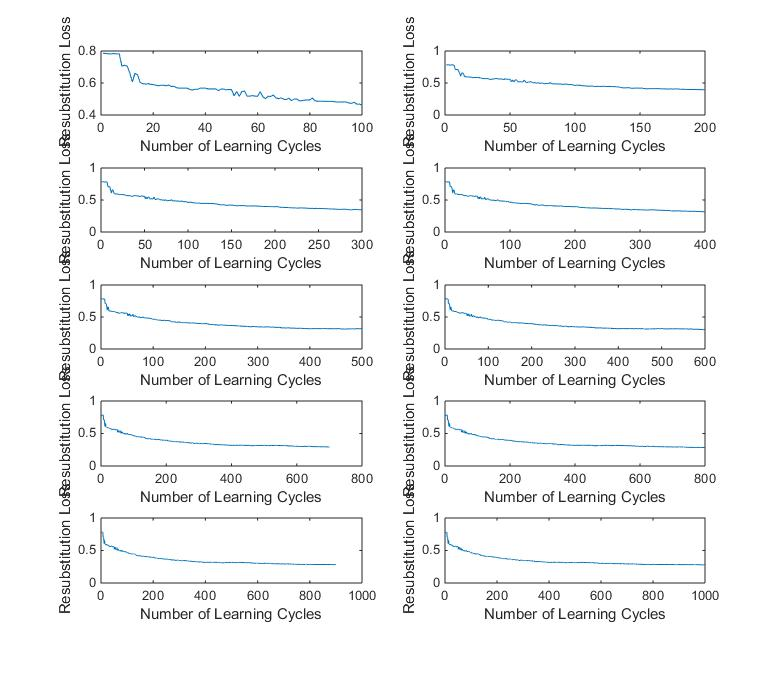
\includegraphics[width=6.5in]{boosting}
% where an .eps filename suffix will be assumed under latex, 
% and a .pdf suffix will be assumed for pdflatex; or what has been declared
% via \DeclareGraphicsExtensions.
%\caption{Simulation Results.}
%\label{fig_sim}
\end{figure}

  \newpage
 
\section{Gaussian Process Classification}

\subsection{Introduction}

The tests were carried out using the code probided on \url{http://www.gaussianprocess.org/gpml/code/matlab/doc/demoClassification.m}
The figure below displays the plot of the training data points and the test data points using KL inference method, exponential covariance function. and Logistic likelihhod function

\begin{figure}[!t]
\centering
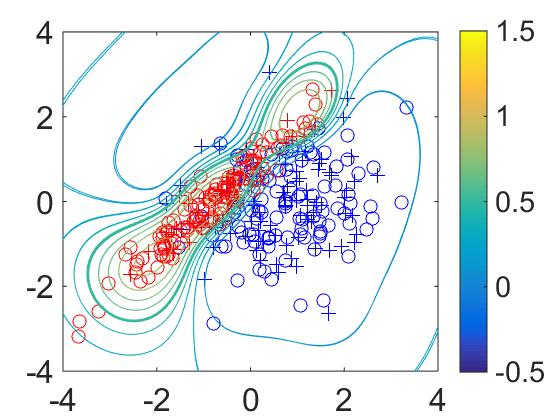
\includegraphics[width=6.5in]{plot11}
% where an .eps filename suffix will be assumed under latex, 
% and a .pdf suffix will be assumed for pdflatex; or what has been declared
% via \DeclareGraphicsExtensions.
%\caption{Simulation Results.}
%\label{fig_sim}
\end{figure}


\subsection{Results}



The classification rate for the test set generated  using the Linear Kernel was found to be 82.73\%, whereas the classification rate for the same test using the squared exponential covariance function was found to be 87.73\%. The histogram of the uncertainities for both the classes is as shown in Figure 1 . When changing the inference method to KL i.e the Kullback-Leibler approximation, the same result i.e 87.73\% was obtained.Changing the likelihood function to Logistic also did not make any signification difference, providing a classification rate of 87.73\%.

\begin{figure*}[!t]
\centering
\subfloat[Correctly Classified]{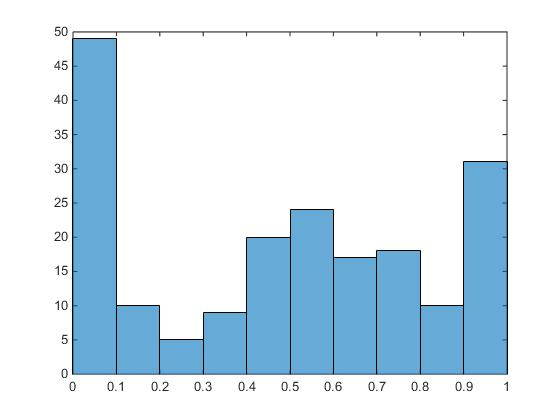
\includegraphics[width=2.5in]{boost1}%
\label{Histogram 1}}
\hfil
\subfloat[Incorrectly Classified]{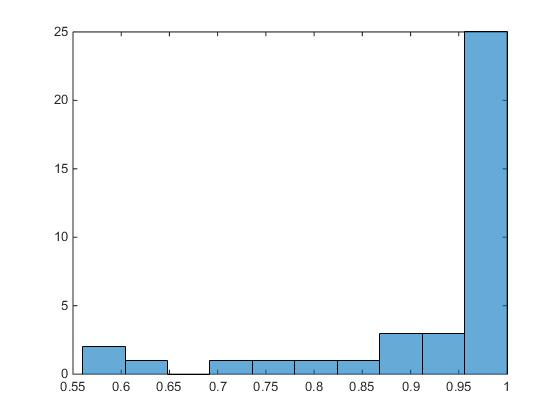
\includegraphics[width=2.5in]{boost2}%
\label{fig_second_case}}
\caption{HISTOGRAM for Gaussian Process.}
\label{fig_sim}
\end{figure*}


Using the Boosting Classifier, for the same set of data points, the following histogram plot was obtained as shown in Figure 2.

\begin{figure*}[!t]
\centering
\subfloat[Correctly Classified]{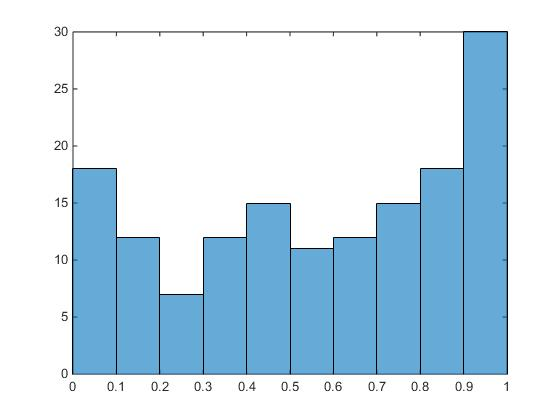
\includegraphics[width=2.5in]{last_linear_boostin1}%
\label{Histogram 1}}
\hfil
\subfloat[Incorrectly Classified]{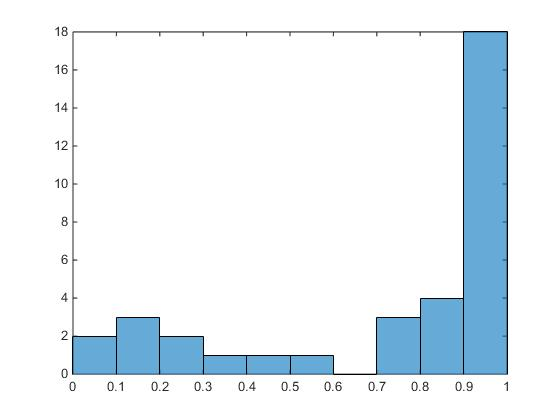
\includegraphics[width=2.5in]{last_linear_boostin2}%
\label{fig_second_case}}
\caption{Histogram for Boosting Classifier.}
\label{fig_sim}
\end{figure*}


\end{document}
